\chapter{Związek z dominowaniem w grafach}
\label{chap:roman_domination}

W niniejszym rozdziale przedstawiono teoretyczne podstawy problemu licencjonowania oprogramowania poprzez przegląd teorii dominowania w grafach. Rozdział zawiera definicje podstawowych pojęć, wprowadza formalizację problemu licencjonowania jako wariantu dominowania rzymskiego oraz analizuje złożoność obliczeniową zagadnienia. Całość stanowi teoretyczne uzasadnienie dla metod algorytmicznych opisanych w dalszej części pracy.

\section{Dominowanie -- podstawowe definicje}
Problematyka dominowania w grafach jest dobrze zbadana i szeroko opisana w literaturze~\cite{haynes1998domination}.
W szczególności znane są klasyczne definicje zbioru dominującego oraz liczby dominowania, które stanowią punkt odniesienia dla dalszych analiz.
Niech $G=(V,E)$ będzie grafem nieskierowanym.
Zbiorem dominującym jest podzbiór $D \subseteq V$ taki, że każdy wierzchołek spoza $D$ ma co najmniej jednego sąsiada w $D$:
\begin{equation}
  \forall v \in V \setminus D \;\; \exists\, u \in D : \{u,v\} \in E ,
  \label{eq:dominating_set_def}
\end{equation}
gdzie:
\begin{itemize}
  \item $V$ - zbiór wierzchołków grafu,
  \item $E$ - zbiór krawędzi grafu,
  \item $D \subseteq V$ - zbiór dominujący,
  \item $u,v \in V$ - wierzchołki grafu,
  \item $\{u,v\}\in E$ - krawędź łącząca wierzchołki $u$ i $v$.
\end{itemize}


Najmniejszą moc zbioru dominującego oznaczamy symbolem $\gamma(G)$ i nazywamy liczbą dominowania:
\begin{equation}
  \gamma(G) = \min \{\, |D| : D \subseteq V \,\},
  \label{eq:domination_number}
\end{equation}
gdzie:
\begin{itemize}
  \item $\gamma(G)$ - liczba dominowania grafu $G$,
  \item $D$ - zbiór dominujący w grafie $G$,
  \item $V$ - zbiór wierzchołków grafu,
  \item $|D|$ - moc zbioru $D$.
\end{itemize}



Z punktu widzenia rozważanego problemu zakupu licencji, podstawowe założenie jest następujące:
jeśli potraktujemy osoby kupujące licencje jako zbiór \(D\), a krawędzie grafu jako relacje
umożliwiające udostępnianie licencji, wówczas warunek dominowania opisany równaniem~(\ref{eq:dominating_set_def}) określa sytuację,
w której każdy użytkownik spoza $D$ ma znajomego w~$D$, a zatem uzyskuje dostęp do usługi.
Gdyby wszystkie licencje były identyczne i pozwalały obsłużyć dowolną liczbę sąsiadów,
minimalizacja kosztu sprowadzałaby się do wyznaczenia liczby dominowania~(\ref{eq:domination_number}).
W praktyce jednak występują różne typy licencji oraz limity
współużytkowników, co czyni problem znacznie bardziej złożonym.

Należy zauważyć, że najmniejszy zbiór dominujący nie musi być jednoznaczny.
W niektórych przypadkach można w grafie znaleźć kilka różnych najmniejszych zbiorów dominujących.
Wynika to bezpośrednio z definicji liczby dominowania~(\ref{eq:domination_number}),
która określa jedynie minimalną moc zbioru dominującego, a nie jego unikalność.
Często graf ma wiele zbiorów dominujących o rozmiarze równym $\gamma(G)$,
jak na rysunku~\ref{fig:dominatingexample}, gdzie trzy zbiory są minimalne względem inkluzji, ale tylko dwa są najmniejsze.
Problem znajdowania $\gamma(G)$ jest jednak dobrze określony i należy do klasy problemów NP-trudnych. Jego wersja decyzyjna sformułowana jest następująco: dla zadanego grafu $G$ oraz liczby całkowitej $k$ pytamy, czy istnieje zbiór dominujący o rozmiarze co najwyżej $k$. Jest to klasyczny problem NP-zupełny \cite{POUREIDI2023106363, PANDA2023337}. Oznacza to, że najprawdopodobniej (przy założeniu $P \neq NP$) nie istnieje algorytm wielomianowy rozwiązujący ten problem w ogólności. W praktyce stosuje się zatem algorytmy przybliżone lub ogranicza analizę do specjalnych klas grafów, dla których problem staje się prostszy. Znane są między innymi efektywne algorytmy zachłanne, które zapewniają rozwiązanie przybliżone z gwarantowanym współczynnikiem. Przykładem jest prosty algorytm zachłanny wybierający kolejno wierzchołki do zbioru dominującego, osiągający przybliżenie rzędu $O(\ln n)$.


\begin{figure}[H]
  \centering
  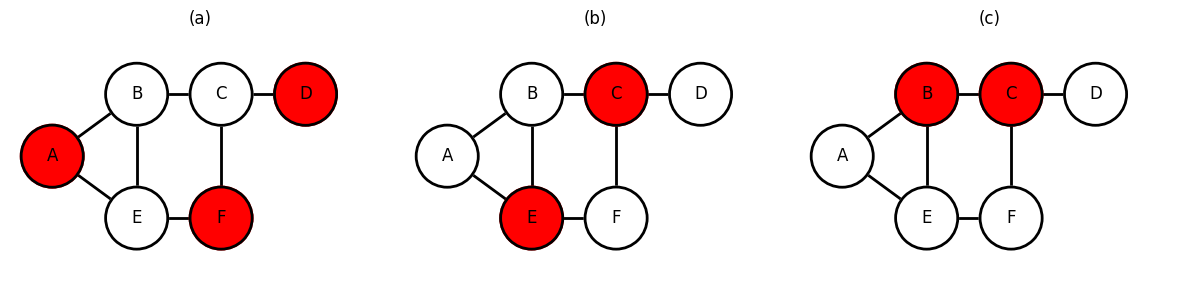
\includegraphics[width=1\textwidth]{assets/dominating-set-example.png}
  \caption[Przykładowe zbiory dominujące]{%
    Przykładowe zbiory dominujące (wyróżnione na czerwono).
    \textbf{(a)}~Minimalny zbiór dominujący o mocy~3.
    \textbf{(b)}-\textbf{(c)}~Dwa różne minimalne i najmniejsze zbiory dominujące, gdzie
    \(\gamma(G)=2\).  Każdy wierzchołek nieczerwony ma sąsiada czerwonego.
  }
  \label{fig:dominatingexample}
\end{figure}

W ogólności nie można poprawić granicy aproksymacji rzędu logarytmicznego. Problem zbioru dominującego jest APX-trudny, a dokładniej log-APX-zupełny \cite{POUREIDI2023106363}. Co więcej, nawet na bardzo ograniczonych grafach, np. grafach o maksymalnym stopniu 3 (grafy kubiczne), problem pozostaje NP-trudny i APX-zupełny \cite{ALIMONTI2000123}. Berman i Fujito (1999) wykazali m.in. NP-trudność pewnych wariantów dominowania w grafach o ograniczonym stopniu \cite{BermanFujitoThreeDegree}, co potwierdza, że zasadnicza trudność problemu dominowania jest obecna już w stosunkowo prostych strukturach.


\section{Dominowanie rzymskie a licencje grupowe}

Dominowanie rzymskie to wariant problemu dominowania, w którym każdemu wierzchołkowi przypisuje się jedną z trzech wartości: 0, 1 lub 2. Wierzchołek o wartości 1 dominuje wyłącznie samego siebie, natomiast wierzchołek o wartości 2 dominuje zarówno siebie, jak i wszystkich swoich sąsiadów. Wymaga się przy tym, aby każdy wierzchołek o wartości 0 był sąsiadem co najmniej jednego wierzchołka oznaczonego wartością 2. Formalnie, funkcja dominowania rzymskiego na grafie $G=(V,E)$ to funkcja $f: V \to \{0,1,2\},$ spełniająca warunek, że dla każdego wierzchołka $v$ z $f(v) = 0$ istnieje sąsiad $u \in V$ taki, że $f(u) = 2$ \cite{Favaron2009}. Minimalizacja sumy wartości $f(v)$ po wszystkich $v \in V$ prowadzi do zdefiniowania tzw. liczby dominowania rzymskiego grafu, oznaczanej $\gamma_R(G)$.

Terminologia i metafora związana z dominowaniem rzymskim wywodzą się z legendy o obronie granic imperium rzymskiego. Zakładano w niej, że w każdej osadzie można umieścić pewną liczbę jednostek wojskowych. Osada z dwiema jednostkami była w stanie bronić się samodzielnie i jednocześnie wysłać wsparcie do sąsiedniej osady. Osada z jedną jednostką broniła wyłącznie siebie, a miejscowości pozbawione jednostek militarnych wymagały ochrony z zewnątrz. W tej metaforze graf reprezentuje system osad i połączeń między nimi, a etykiety 0, 1 i 2 odpowiadają decyzjom o rozmieszczeniu wojsk. Koncepcję dominowania rzymskiego wprowadzili do teorii grafów Cockayne i współpracownicy w 2004 roku \cite{Cockayne2004}.


W kontekście problemu optymalnego zakupu licencji w grafach reprezentujących sieci społecznościowe interpretacja jest bezpośrednia. Wartość $f(v)=2$ odpowiada użytkownikowi $v$, który nabywa licencję grupową i zapewnia dostęp zarówno sobie, jak i co najmniej jednemu ze swoich sąsiadów. Wartość $f(v)=1$ oznacza użytkownika posiadającego licencję indywidualną, pokrywającą wyłącznie jego samego. Natomiast $f(v)=0$ reprezentuje użytkownika bez własnej licencji, który musi polegać na pokryciu przez sąsiada z wartością 2. Warunek dominowania rzymskiego, zgodnie z którym każdy wierzchołek z etykietą 0 ma sąsiada z etykietą 2, gwarantuje dokładnie to, co w naszym modelu jest wymagane: każdy użytkownik bez licencji ma znajomego z licencją grupową, który może podzielić się z nim dostępem. W ten sposób każda funkcja $f:V \to \{0,1,2\}$ spełniająca warunki dominowania rzymskiego wyznacza dopuszczalną strategię licencyjną w rozważanej sieci.


Waga funkcji dominowania rzymskiego definiowana jest jako $w(f) = \sum_{v \in V} f(v)$, czyli suma przypisanych wartości. Liczba dominowania rzymskiego $\gamma_R(G)$ to najmniejsza możliwa waga funkcji dominowania rzymskiego dla grafu $G$. Jeśli przyjmiemy, że koszt licencji indywidualnej wynosi 1, a grupowej 2, to minimalizacja kosztu w naszym problemie pokrywa się z zagadnieniem znalezienia funkcji dominowania rzymskiego o najmniejszej wadze. Cel minimalizacji całkowitego kosztu $C = |I| + 2|H|$ jest równoważny minimalizacji $w(f)$, gdy $|I|$ utożsamimy z liczbą wierzchołków o etykiecie 1, a $|H|$ z liczbą wierzchołków o etykiecie 2. Należy jednak podkreślić, że pełna równoważność z dominowaniem rzymskim zachodzi tylko wtedy, gdy liczba sąsiadów dowolnego wierzchołka nie przekracza maksymalnej liczby użytkowników dopuszczonych w planie grupowym. Jak wspomniano wcześniej przy omawianiu parametrów $m$ i $k$, nasze ujęcie wprowadza dodatkowe ograniczenie pojemności -- wierzchołek dla którego funkcja $f$ przyjmuje wartość 2 może pokrywać jedynie ograniczoną liczbę sąsiadów. Problem optymalnego zakupu licencji jest więc uogólnieniem dominowania rzymskiego, dostosowanym do praktycznych limitów występujących w planach subskrypcyjnych.

W przypadku innych modeli cenowych, dominowanie rzymskie stanowi nadal użyteczną metaforę, choć nie oddaje w sposób wystarczający struktury kosztów. 
Stosunek kosztu licencji grupowej do indywidualnej oznaczamy przez $p_r = c_g / c_i$. W klasycznym dominowaniu rzymskim przyjmuje się, że $p_r=2$, co odpowiada sytuacji, w której licencja grupowa kosztuje dokładnie dwukrotnie więcej niż indywidualna.
Gdy $p_r \neq 2$, możemy rozważyć ogólniejsze przypisania wag, w których etykieta odpowiada rzeczywistemu kosztowi planu. Przykładowo, gdy $p_r=3$, to licencja grupowa ma koszt równy trzem jednostkom, co nie mieści się w klasycznym schemacie $\{0,1,2\}$. W literaturze zaproponowano rozszerzenia pozwalające modelować podobone sytuacje, m.in. $k$-dominowanie rzymskie, gdzie dopuszcza się wartości $\{0,1,\dots,k\}$ \cite{CHAUDHARY2024301}, czy też dominowanie rzymskie z wagami \cite{Ghaffari2020}. Warianty te pozwalają odwzorować przypadki, w których dostępne są plany o różnych kosztach i różnej pojemności, np. licencja droższa, ale umożliwiająca współdzielenie w większej grupie. W tym sensie uogólnienia dominowania rzymskiego są bliższe rzeczywistemu problemowi optymalizacji kosztów licencji niż klasyczna wersja ograniczona do wartości 0, 1 i 2.

Na potrzeby tej pracy nie jest jednak konieczne wchodzenie w szczegółowe odmiany dominowania rzymskiego. Wystarczy zauważyć, że w analizowanym modelu schemat pozostaje taki sam jak w klasycznej wersji, a jedyną różnicą jest koszt przypisywany wierzchołkom o etykiecie $2$. W zależności od przyjętego modelu cenowego wartość ta może wynosić np. $p_r=1.5$, $p_r=2.5$ lub $p_r=3$. Konstrukcja funkcji dominowania rzymskiego oraz sam podział na etykiety $\{0,1,2\}$ nie ulega zmianie. Innymi słowy, dominowanie rzymskie dostarcza prostego i intuicyjnego opisu sytuacji.

Prosty przykład zastosowania dominowania rzymskiego można przedstawić na grafie typu gwiazda. Centralny wierzchołek $A$ jest połączony z liśćmi $B, C, D, E$. Najlepszą strategią jest, aby $A$ wykupił licencję grupową i udostępnił ją wszystkim swoim sąsiadom. W modelu oznacza to $f(A)=2$, a dla każdego liścia $f(B)=f(C)=f(D)=f(E)=0$. Warunek dominowania rzymskiego jest spełniony, ponieważ każdy liść, dla którego $f=0$, ma sąsiada $A$ z $f=2$. Waga funkcji wynosi wówczas $w(f)=2$ - odpowiada to kosztowi jednej licencji grupowej obsługującej całą pięcioosobową grupę.

Dla porównania można rozważyć inne strategie. Gdyby każdy wierzchołek nabył licencję indywidualną, wówczas $w(f)=5$, co odpowiada kosztowi pięciu licencji indywidualnych. Jeśli centralny wierzchołek nabyłby wyłącznie licencję indywidualną ($f(A)=1$), a liście pozostałyby bez dostępu ($f(B)=f(C)=f(D)=f(E)=0$), warunek nie byłby spełniony, ponieważ żaden liść nie miałby sąsiada przyjmującego dla funkcji $f$ wartość 2.

Rysunek~\ref{fig:romandomatinonstarexamepl} ilustruje przykład i pokazuje, jak dominowanie rzymskie wskazuje optymalny wybór wierzchołka centralnego jako posiadacza licencji grupowej. W większych grafach liczba kandydatów do roli posiadaczy licencji grupowych rośnie, a ich dobór prowadzi do problemu optymalizacji funkcji dominowania rzymskiego.


\begin{figure}[H]
  \centering
  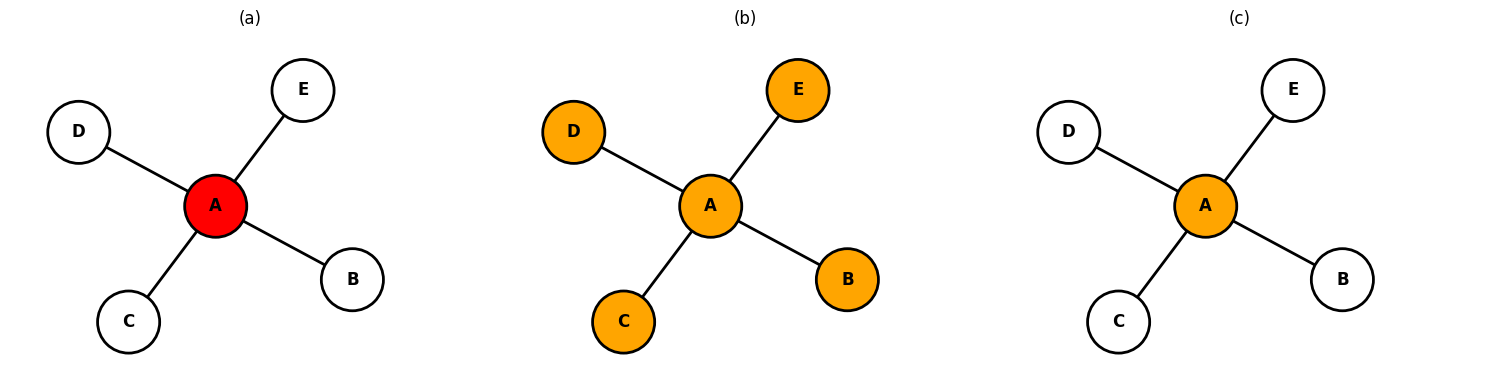
\includegraphics[width=1\textwidth]{assets/stars.png}
  \caption{
  Przykład dominowania rzymskiego na grafie typu gwiazda.  
  Kolory: biały = $f(v)=0$, pomarańczowy = $f(v)=1$, czerwony = $f(v)=2$.
    \textbf{(a)}~Przypisanie optymalne ($w(f)=2$).
    \textbf{(b)}~$f(A)=f(B)=f(C)=f(D)=f(E)=1$ ($w(f)=5$).
    \textbf{(c)}~$f(A)=1$, liście $f(B)=f(C)=f(D)=f(E)=0$ (niespełniony warunek).
  }
  \label{fig:romandomatinonstarexamepl}
\end{figure}


\section{Złożoność obliczeniowa problemu}

Dokładne dowody z zakresu złożoności obliczeniowej znajdują się w literaturze; wykazano NP-zupełność problemu dominowania rzymskiego m.in. przez redukcję z problemu pokrycia wierzchołków lub zbioru dominującego \cite{chambers2009}. W kontekście naszego modelu oznacza to, że optymalne wyznaczenie użytkowników kupujących poszczególne licencje jest obliczeniowo trudne dla dużych sieci. Innymi słowy, nie istnieje znany algorytm wielomianowy, który gwarantowałby znalezienie rozwiązania minimalnego kosztu dla dowolnej struktury grafu znajomości - w najgorszym przypadku liczba kombinacji rośnie wykładniczo wraz z liczbą wierzchołków.

Konsekwencją NP-trudności jest także brak prostego schematu aproksymacyjnego dla problemu minimalizacji kosztów licencji. Ponieważ problem dominowania (minimalnego zbioru dominującego) jest APX-zupełny (dla konkretnych rodzajów grafów) \cite{POUREIDI2023106363}, nie ma wielomianowego schematu aproksymacji (PTAS) gwarantującego dobre przybliżenie. Dla naszego problemu, który uogólnia dominowanie, obowiązują podobne ograniczenia; w najgorszym przypadku nie uzyska się w czasie wielomianowym przybliżenia lepszego niż rzędu $O(\ln n)$. Proste heurystyki zachłanne mogą jednak dawać przyzwoite wyniki. Przykładowo heurystyka wybierająca iteracyjnie wierzchołek pokrywający najwięcej niepokrytych sąsiadów (z przypisaniem licencji grupowej) realizuje algorytm zachłanny i osiąga współczynnik co najwyżej $2+\ln \Delta$, gdzie $\Delta$ to maksymalny stopień grafu \cite{Kuhn2012NetworkAlgorithms}. W najgorszym przypadku jest to $O(\ln n)$, natomiast w praktyce wyniki bywają lepsze od tej granicy. Problem pozostaje trudny także dla grafów o niewielkich stopniach; dla grafów o stopniu co najwyżej cztery wyznaczenie najmniejszego zbioru dominującego jest APX-zupełne \cite{ALIMONTI2000123,POUREIDI2023106363}.
Wynika stąd, że ograniczenie maksymalnej liczby sąsiadów nie upraszcza problemu do trywialnego. Nawet w sieciach o małym stopniu optymalny przydział do licencji grupowych może wymagać złożonych obliczeń.

W dalszej części pracy nacisk położono na podejścia algorytmiczne uwzględniające tę złożoność. Przyjęto podejście dwutorowe: (a) zastosowanie metod dokładnych dla umiarkowanych rozmiarów sieci oraz (b) projektowanie i analizę algorytmów heurystycznych dostarczających dobre rozwiązania dla większych sieci. W literaturze można już znaleźć próby wykorzystania technik optymalizacyjnych do problemu dominowania; przykładem jest praca Parra Inza i współautorów \cite{PARRAINZA2024926}, w której zagadnienie sformułowano jako ILP i uzupełniono heurystykami naprawczymi. Tego typu konstrukcję można zaadaptować do omawianego problemu, wprowadzając zmienne decyzyjne wskazujące wybór typu licencji dla każdego użytkownika oraz odpowiednie ograniczenia. Algorytmy zachłanne, metody lokalnego przeszukiwania oraz metaheurystyki, np. algorytmy genetyczne czy symulowane wyżarzanie, pozwalają szybko przeszukiwać przestrzeń możliwych konfiguracji licencji.

\section{Podsumowanie}

W niniejszym rozdziale przedstawiono teoretyczne podstawy problemu licencjonowania oprogramowania w kontekście teorii dominowania w grafach. Kluczowym wnioskiem jest identyfikacja problemu jako wariantu dominowania rzymskiego, gdzie węzły mogą przyjmować różne typy licencji odpowiadające stanowi niezabezpieczonemu, zabezpieczonemu przez sąsiada lub będącemu właścicielem licencji grupowej.

Analiza złożoności obliczeniowej wykazała NP-trudność problemu, co wynika bezpośrednio z redukcji z klasycznego problemu zbioru dominującego. Konsekwencją tej właściwości jest brak wielomianowego algorytmu dokładnego oraz ograniczona jakość aproksymacji -- w najgorszym przypadku nie można uzyskać w czasie wielomianowym przybliżenia lepszego niż $O(\ln n)$. Problem pozostaje trudny nawet dla grafów o ograniczonym stopniu, co oznacza, że ograniczenie maksymalnej liczby sąsiadów nie upraszcza zagadnienia do trywialnego.

Ustalenie związku z dominowaniem rzymskim dostarcza solidnych podstaw teoretycznych dla konstrukcji algorytmów dokładnych i heurystycznych. W szczególności umożliwia to adaptację znanych metod optymalizacyjnych, takich jak programowanie całkowitoliczbowe, oraz projektowanie heurystyk wykorzystujących właściwości strukturalne grafów. Przedstawione rezultaty stanowią fundament dla dalszych analiz algorytmicznych oraz eksperymentów empirycznych opisanych w kolejnych rozdziałach.
